Fixed points and (known) conserved quantites for the concentric, axis-parallel (CAP) families of \cref{sec:03-other-conc} appear in
\cref{tab:n3-conc-families}. Those for the non-concentric (NCAP) families of \cref{sec:03-non-conc} appear in
\cref{tab:n3-non-conc-families}. A diagram appears in \cref{fig:03-transformations} which illustrate how certain pairs of families are interrelated by either similarity or polar transformations.

\begin{table}
\centering
\begin{tabular}{|r|c|c|l|}
\hline
Family & Fixed & Conserves & Notes \\
\hline
\makecell[rc]{Poristic\\(bicentric)} & $X_1$, $X_3$, $X_{40}$, $\ldots$ & $\sum\cos\theta_i,a_9/b_9$ & \makecell[lc]{polar image of Confocal family\\wrt to a focus} \\
\hline
\makecell[rt]{Poristic\\Excentrals} & $X_2$, $X_3$, $X_4$, $X_5$ & $\sum{s_i^2}$, $\prod\cos\theta_i$ & \makecell[lt]{Inscribed in circle;\\caustic is MacBeath inconic} \\
\hline
Brocard & \makecell[lc]{$X_3$, $X_6$, $X_{15}$, $X_{16}$,\\$X_{39}$, $X_{182},\ldots$,\\$\Omega_1$, $\Omega_2$} & $\sum{s_i^{-2}}$, $\omega$, $\sum\cot\theta_i$ & \makecell[lc]{polar image of Homothetic\\family wrt caustic focus;\\inscribed in circle;\\caustic is Brocard inellipse}\\
%\hline
%focus-Inversive & $X_7$ & $L,\sum\cos\theta_i$ & \makecell[lc]{inversive image of Confocals\\wrt a focus; non-Ponceletian;\\inscribed in Pascal's limaçon;\\caustic non-ellipse}\\
\hline
\end{tabular}
\caption{Summary of fixed points and (known) conserved quantites for the non-concentric, axis-parallel (NCAP) families of \cref{sec:03-non-conc}.}
\label{tab:n3-non-conc-families}
\end{table}

\begin{figure}
    \centering
    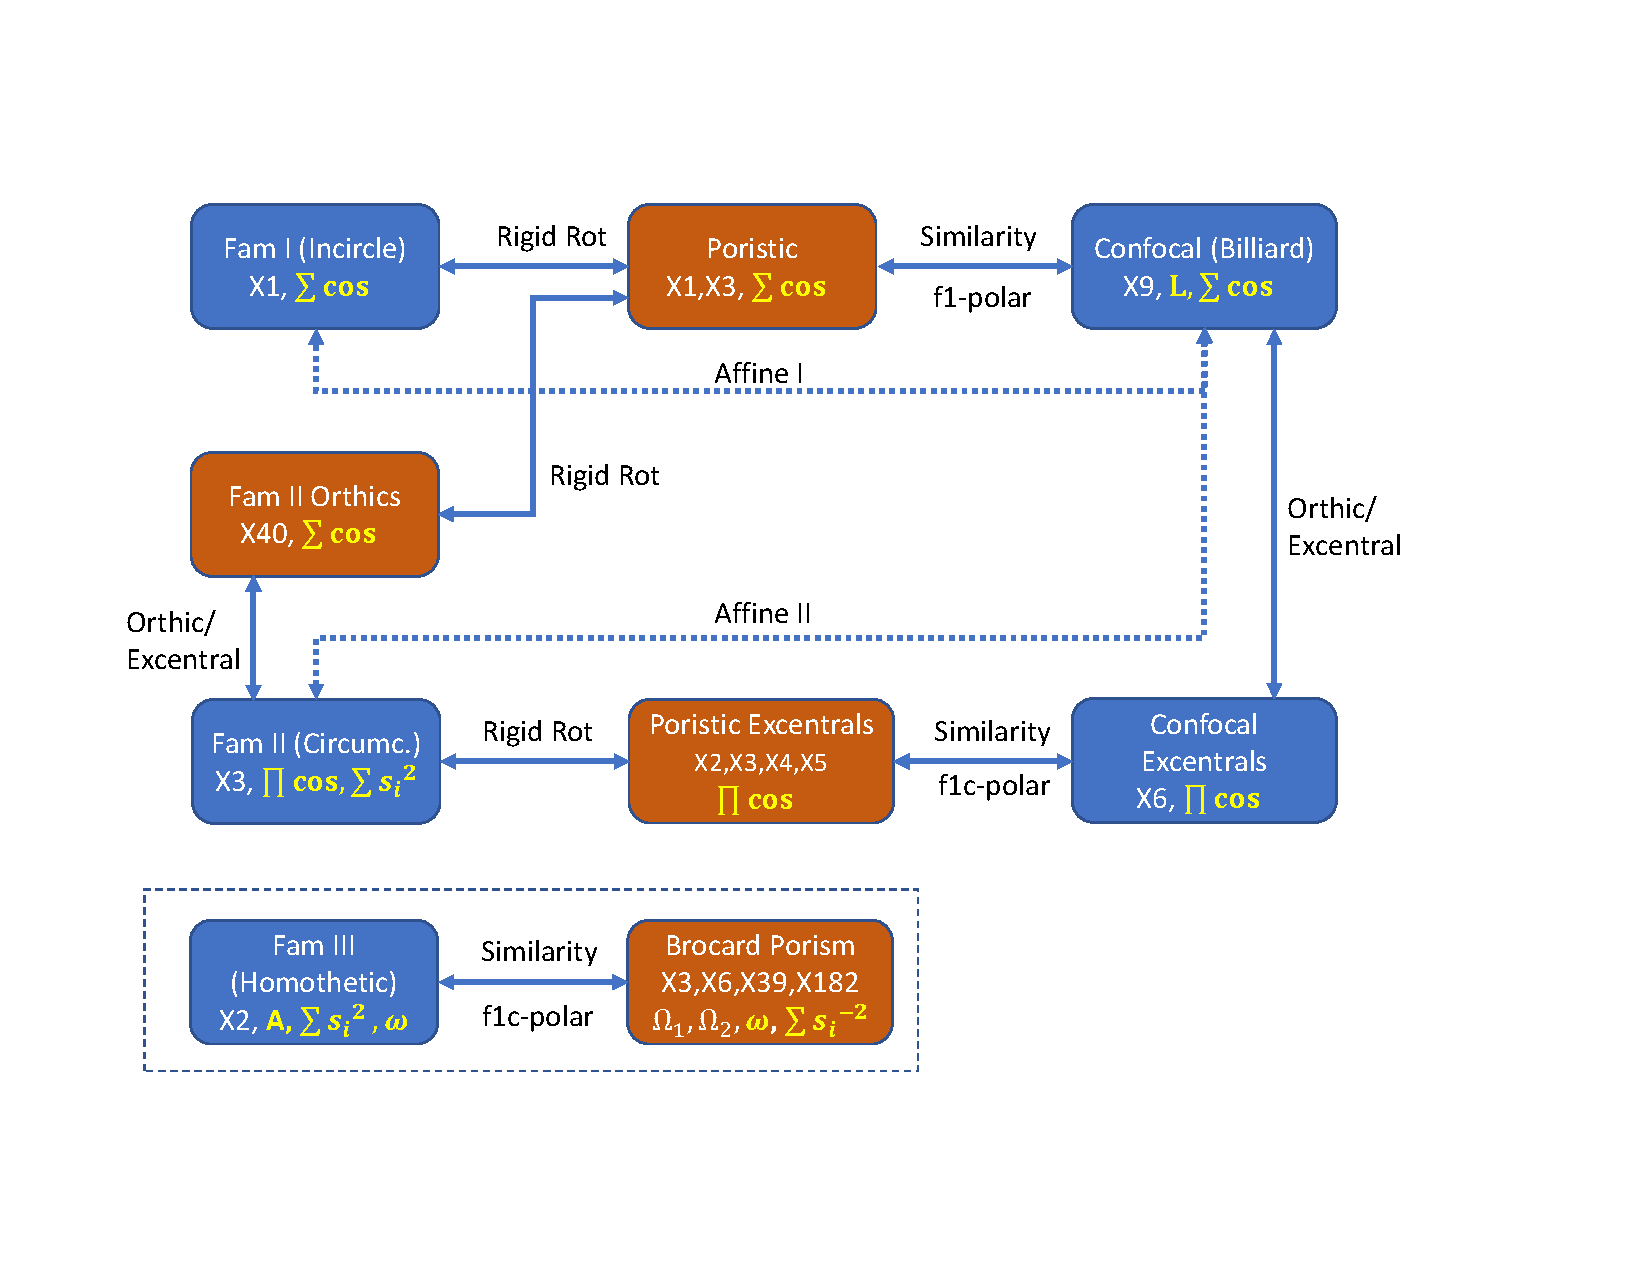
\includegraphics[width=\textwidth]{pics_03_250_poncelet_transformations.pdf}
  \caption{Families mentioned in this chapter (blue ones are concentric, tan ones are non-concentric), as well as the transformations under which certain families are interrelated.}
    \label{fig:03-transformations}
\end{figure}

\subsection{Invariants preserved when \torp{$N>3$}{N>3}}

\cref{tab:03-summary} summarizes some properties of 3-periodics mentioned herein. The last column reveals that many of the invariants continue to hold for N>3. 

\begin{table}
\begin{tabular}{|l|l|l|l|l|l|}
\hline
fam. & pair & \makecell[lt]{N=3\\outer conic} & \makecell[lt]
{N=3\\inner conic} & \makecell[lt]{N=3\\invariants} & \makecell[lt]{N>3} \\
\hline
 & billiard & ellipse $(a,b)$ & confocal caustic & $L,J,r/R,\color{red}\sum\cos$ & $L,J,\color{red}\sum\cos$ \\
I & inner circle & ellipse $(a,b)$ & circle $r=\frac{{a}{b}}{a+b}$ & $R,r/R,\color{red}\sum\cos$ & $\color{red}\sum\cos$ \\
II & outer circle & $R=(a+b)$ & ellipse $(a,b)$ & $\sum{s_i^2},\color{red}\prod\cos$ & $\sum{s_i^2},\color{red}\prod\cos$ \\
III & homothetic & ellipse $(a,b)$ & ellipse $(a/2,b/2)$ & $A,\sum{s_i^2},\omega,\color{red}\sum\cot$ & $A,\sum{s_i^2},\color{red}\sum\cot$ \\
%4 & $X_4$ stationary & ellipse $(a,b)$ & ellipse $(a_0,b_0)$ & $X_4=0$ & pseudo-$X_4$ = 0 \\
\hline
\end{tabular}
\caption{Summary of properties across different concentric Poncelet families. The last column shows some invariants which continue to hold for N>3.}
\label{tab:03-summary}
\end{table}
